\documentclass[twoside]{book}

% Packages required by doxygen
\usepackage{fixltx2e}
\usepackage{calc}
\usepackage{doxygen}
\usepackage[export]{adjustbox} % also loads graphicx
\usepackage{graphicx}
\usepackage[utf8]{inputenc}
\usepackage{makeidx}
\usepackage{multicol}
\usepackage{multirow}
\PassOptionsToPackage{warn}{textcomp}
\usepackage{textcomp}
\usepackage[nointegrals]{wasysym}
\usepackage[table]{xcolor}

% Font selection
\usepackage[T1]{fontenc}
\usepackage[scaled=.90]{helvet}
\usepackage{courier}
\usepackage{amssymb}
\usepackage{sectsty}
\renewcommand{\familydefault}{\sfdefault}
\allsectionsfont{%
  \fontseries{bc}\selectfont%
  \color{darkgray}%
}
\renewcommand{\DoxyLabelFont}{%
  \fontseries{bc}\selectfont%
  \color{darkgray}%
}
\newcommand{\+}{\discretionary{\mbox{\scriptsize$\hookleftarrow$}}{}{}}

% Page & text layout
\usepackage{geometry}
\geometry{%
  a4paper,%
  top=2.5cm,%
  bottom=2.5cm,%
  left=2.5cm,%
  right=2.5cm%
}
\tolerance=750
\hfuzz=15pt
\hbadness=750
\setlength{\emergencystretch}{15pt}
\setlength{\parindent}{0cm}
\setlength{\parskip}{3ex plus 2ex minus 2ex}
\makeatletter
\renewcommand{\paragraph}{%
  \@startsection{paragraph}{4}{0ex}{-1.0ex}{1.0ex}{%
    \normalfont\normalsize\bfseries\SS@parafont%
  }%
}
\renewcommand{\subparagraph}{%
  \@startsection{subparagraph}{5}{0ex}{-1.0ex}{1.0ex}{%
    \normalfont\normalsize\bfseries\SS@subparafont%
  }%
}
\makeatother

% Headers & footers
\usepackage{fancyhdr}
\pagestyle{fancyplain}
\fancyhead[LE]{\fancyplain{}{\bfseries\thepage}}
\fancyhead[CE]{\fancyplain{}{}}
\fancyhead[RE]{\fancyplain{}{\bfseries\leftmark}}
\fancyhead[LO]{\fancyplain{}{\bfseries\rightmark}}
\fancyhead[CO]{\fancyplain{}{}}
\fancyhead[RO]{\fancyplain{}{\bfseries\thepage}}
\fancyfoot[LE]{\fancyplain{}{}}
\fancyfoot[CE]{\fancyplain{}{}}
\fancyfoot[RE]{\fancyplain{}{\bfseries\scriptsize Generated by Doxygen }}
\fancyfoot[LO]{\fancyplain{}{\bfseries\scriptsize Generated by Doxygen }}
\fancyfoot[CO]{\fancyplain{}{}}
\fancyfoot[RO]{\fancyplain{}{}}
\renewcommand{\footrulewidth}{0.4pt}
\renewcommand{\chaptermark}[1]{%
  \markboth{#1}{}%
}
\renewcommand{\sectionmark}[1]{%
  \markright{\thesection\ #1}%
}

% Indices & bibliography
\usepackage{natbib}
\usepackage[titles]{tocloft}
\setcounter{tocdepth}{3}
\setcounter{secnumdepth}{5}
\makeindex

% Hyperlinks (required, but should be loaded last)
\usepackage{ifpdf}
\ifpdf
  \usepackage[pdftex,pagebackref=true]{hyperref}
\else
  \usepackage[ps2pdf,pagebackref=true]{hyperref}
\fi
\hypersetup{%
  colorlinks=true,%
  linkcolor=blue,%
  citecolor=blue,%
  unicode%
}

% Custom commands
\newcommand{\clearemptydoublepage}{%
  \newpage{\pagestyle{empty}\cleardoublepage}%
}

\usepackage{caption}
\captionsetup{labelsep=space,justification=centering,font={bf},singlelinecheck=off,skip=4pt,position=top}

%===== C O N T E N T S =====

\begin{document}

% Titlepage & ToC
\hypersetup{pageanchor=false,
             bookmarksnumbered=true,
             pdfencoding=unicode
            }
\pagenumbering{alph}
\begin{titlepage}
\vspace*{7cm}
\begin{center}%
{\Large Heis-\/prosjekt }\\
\vspace*{1cm}
{\large Generated by Doxygen 1.8.13}\\
\end{center}
\end{titlepage}
\clearemptydoublepage
\pagenumbering{roman}
\tableofcontents
\clearemptydoublepage
\pagenumbering{arabic}
\hypersetup{pageanchor=true}

%--- Begin generated contents ---
\chapter{Data Structure Index}
\section{Data Structures}
Here are the data structures with brief descriptions\+:\begin{DoxyCompactList}
\item\contentsline{section}{\hyperlink{structelevator}{elevator} \\*A structure to represent the elevator. Contains memory of current state, queue of orders and time, as well as current and previous floor and direction }{\pageref{structelevator}}{}
\end{DoxyCompactList}

\chapter{File Index}
\section{File List}
Here is a list of all documented files with brief descriptions\+:\begin{DoxyCompactList}
\item\contentsline{section}{source/{\bfseries elevator.\+c} }{\pageref{elevator_8c}}{}
\item\contentsline{section}{source/\hyperlink{elevator_8h}{elevator.\+h} \\*Provides communication between the elevator and the hardware }{\pageref{elevator_8h}}{}
\item\contentsline{section}{source/{\bfseries fsm.\+c} }{\pageref{fsm_8c}}{}
\item\contentsline{section}{source/\hyperlink{fsm_8h}{fsm.\+h} \\*The finite state machine }{\pageref{fsm_8h}}{}
\item\contentsline{section}{source/\hyperlink{hardware_8h}{hardware.\+h} \\*Driver for the elevator hardware }{\pageref{hardware_8h}}{}
\item\contentsline{section}{source/{\bfseries main.\+c} }{\pageref{main_8c}}{}
\item\contentsline{section}{source/{\bfseries queue.\+c} }{\pageref{queue_8c}}{}
\item\contentsline{section}{source/\hyperlink{queue_8h}{queue.\+h} \\*Takes care of the elevator\textquotesingle{}s queue }{\pageref{queue_8h}}{}
\item\contentsline{section}{source/\hyperlink{states_8h}{states.\+h} \\*Creates a struct for the elevator and an enumerator for its different states }{\pageref{states_8h}}{}
\item\contentsline{section}{source/{\bfseries timer.\+c} }{\pageref{timer_8c}}{}
\item\contentsline{section}{source/\hyperlink{timer_8h}{timer.\+h} \\*Functions to keep the door open for a period of time }{\pageref{timer_8h}}{}
\item\contentsline{section}{source/driver/{\bfseries channels.\+h} }{\pageref{channels_8h}}{}
\item\contentsline{section}{source/driver/{\bfseries hardware\+\_\+sal.\+c} }{\pageref{hardware__sal_8c}}{}
\item\contentsline{section}{source/driver/{\bfseries hardware\+\_\+sim.\+c} }{\pageref{hardware__sim_8c}}{}
\item\contentsline{section}{source/driver/{\bfseries io.\+c} }{\pageref{io_8c}}{}
\item\contentsline{section}{source/driver/{\bfseries io.\+h} }{\pageref{io_8h}}{}
\end{DoxyCompactList}

\chapter{Data Structure Documentation}
\hypertarget{structelevator}{}\section{elevator Struct Reference}
\label{structelevator}\index{elevator@{elevator}}


A structure to represent the elevator. Contains memory of current state, queue of orders and time, as well as current and previous floor and direction.  




{\ttfamily \#include $<$states.\+h$>$}

\subsection*{Data Fields}
\begin{DoxyCompactItemize}
\item 
\mbox{\Hypertarget{structelevator_acb09243d4d09143920731df452b1ed02}\label{structelevator_acb09243d4d09143920731df452b1ed02}} 
\hyperlink{states_8h_a09fd0473240586cf26c56b9c75589073}{elev\+\_\+state} {\bfseries state}
\item 
\mbox{\Hypertarget{structelevator_ae311bf8256d89166baf4a0017507ae5c}\label{structelevator_ae311bf8256d89166baf4a0017507ae5c}} 
int {\bfseries previousfloor}
\item 
\mbox{\Hypertarget{structelevator_a24496bfa1eacfdec1475e3ae3e6e73f5}\label{structelevator_a24496bfa1eacfdec1475e3ae3e6e73f5}} 
int {\bfseries currentfloor}
\item 
\mbox{\Hypertarget{structelevator_aaf598f7465fc2e79630d9127ef6c8683}\label{structelevator_aaf598f7465fc2e79630d9127ef6c8683}} 
int {\bfseries queue} \mbox{[}H\+A\+R\+D\+W\+A\+R\+E\+\_\+\+N\+U\+M\+B\+E\+R\+\_\+\+O\+F\+\_\+\+F\+L\+O\+O\+RS\mbox{]}\mbox{[}H\+A\+R\+D\+W\+A\+R\+E\+\_\+\+N\+U\+M\+B\+E\+R\+\_\+\+O\+F\+\_\+\+B\+U\+T\+T\+O\+NS\mbox{]}
\item 
\mbox{\Hypertarget{structelevator_a98f9e9d9e81effe445ff82d8e86a60c5}\label{structelevator_a98f9e9d9e81effe445ff82d8e86a60c5}} 
\hyperlink{hardware_8h_a2167c399a24df296afc432bcb88228af}{Hardware\+Movement} {\bfseries previous\+\_\+dir}
\item 
\mbox{\Hypertarget{structelevator_a5bd0a30b0bb1258fac8e6ffeef258338}\label{structelevator_a5bd0a30b0bb1258fac8e6ffeef258338}} 
\hyperlink{hardware_8h_a2167c399a24df296afc432bcb88228af}{Hardware\+Movement} {\bfseries current\+\_\+dir}
\item 
\mbox{\Hypertarget{structelevator_af0715c7b366082e0edbe4dd8f7d755a0}\label{structelevator_af0715c7b366082e0edbe4dd8f7d755a0}} 
time\+\_\+t {\bfseries start\+\_\+time}
\end{DoxyCompactItemize}


\subsection{Detailed Description}
A structure to represent the elevator. Contains memory of current state, queue of orders and time, as well as current and previous floor and direction. 

Definition at line 33 of file states.\+h.



The documentation for this struct was generated from the following file\+:\begin{DoxyCompactItemize}
\item 
source/\hyperlink{states_8h}{states.\+h}\end{DoxyCompactItemize}

\chapter{File Documentation}
\hypertarget{elevator_8h}{}\section{source/elevator.h File Reference}
\label{elevator_8h}\index{source/elevator.\+h@{source/elevator.\+h}}


Provides communication between the elevator and the hardware.  


{\ttfamily \#include $<$stdio.\+h$>$}\newline
{\ttfamily \#include $<$stdlib.\+h$>$}\newline
{\ttfamily \#include $<$signal.\+h$>$}\newline
{\ttfamily \#include \char`\"{}hardware.\+h\char`\"{}}\newline
{\ttfamily \#include \char`\"{}queue.\+h\char`\"{}}\newline
Include dependency graph for elevator.\+h\+:\nopagebreak
\begin{figure}[H]
\begin{center}
\leavevmode
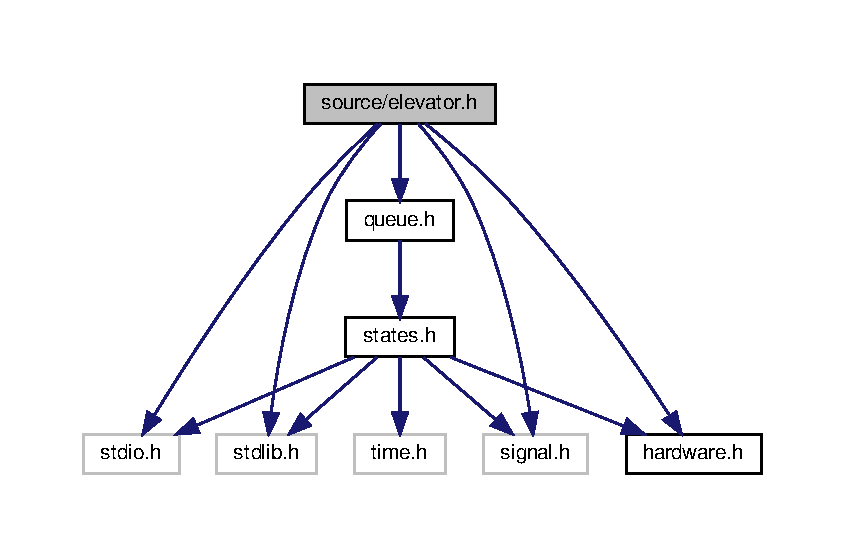
\includegraphics[width=350pt]{elevator_8h__incl}
\end{center}
\end{figure}
This graph shows which files directly or indirectly include this file\+:\nopagebreak
\begin{figure}[H]
\begin{center}
\leavevmode
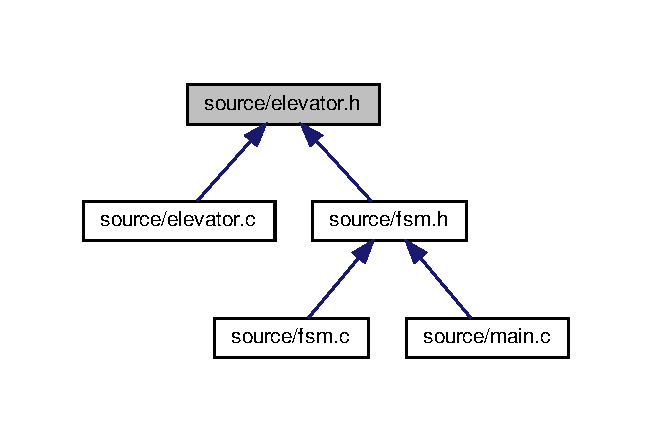
\includegraphics[width=313pt]{elevator_8h__dep__incl}
\end{center}
\end{figure}
\subsection*{Functions}
\begin{DoxyCompactItemize}
\item 
int \hyperlink{elevator_8h_a6dc30b1815d08f01375368de9a48b9b0}{elev\+\_\+get\+\_\+current\+\_\+floor} ()
\begin{DoxyCompactList}\small\item\em Gets the current floor. \end{DoxyCompactList}\item 
void \hyperlink{elevator_8h_a6ecc6ecec304caf35ed5316556009a7f}{elev\+\_\+set\+\_\+current\+\_\+floor} (\hyperlink{structelevator}{elevator} $\ast$el)
\begin{DoxyCompactList}\small\item\em Sets the current floor when the elevator arrives at a new floor. \end{DoxyCompactList}\item 
void \hyperlink{elevator_8h_ac0e8478b1c283ca752a60dab249a7b69}{elev\+\_\+set\+\_\+floor\+\_\+indicator} (\hyperlink{structelevator}{elevator} $\ast$el)
\begin{DoxyCompactList}\small\item\em Sets the floor indicator light for the current floor. If the elevator is between floors, the floor indicator light is lit for the previous floor. \end{DoxyCompactList}\item 
\hyperlink{hardware_8h_a2167c399a24df296afc432bcb88228af}{Hardware\+Movement} \hyperlink{elevator_8h_a4211046ff062aaa48cf6355059ba282d}{elev\+\_\+set\+\_\+motor\+\_\+dir} (\hyperlink{structelevator}{elevator} $\ast$el)
\begin{DoxyCompactList}\small\item\em Sets the motor direction depending on previous direction and next orders. \end{DoxyCompactList}\item 
void \hyperlink{elevator_8h_a79c037675197b1bed2ebb4f4f7d10a74}{elev\+\_\+update\+\_\+dir} (\hyperlink{structelevator}{elevator} $\ast$el)
\begin{DoxyCompactList}\small\item\em Updates previous and current direction. \end{DoxyCompactList}\item 
void \hyperlink{elevator_8h_a01cb37f9f851a7b6d21f166d843aabb7}{elev\+\_\+control\+\_\+range} (\hyperlink{structelevator}{elevator} $\ast$el)
\begin{DoxyCompactList}\small\item\em Secures that the elevator does not move past its range by changing the motor direction when it reaches the top/bottom floor. \end{DoxyCompactList}\end{DoxyCompactItemize}


\subsection{Detailed Description}
Provides communication between the elevator and the hardware. 



\subsection{Function Documentation}
\mbox{\Hypertarget{elevator_8h_a01cb37f9f851a7b6d21f166d843aabb7}\label{elevator_8h_a01cb37f9f851a7b6d21f166d843aabb7}} 
\index{elevator.\+h@{elevator.\+h}!elev\+\_\+control\+\_\+range@{elev\+\_\+control\+\_\+range}}
\index{elev\+\_\+control\+\_\+range@{elev\+\_\+control\+\_\+range}!elevator.\+h@{elevator.\+h}}
\subsubsection{\texorpdfstring{elev\+\_\+control\+\_\+range()}{elev\_control\_range()}}
{\footnotesize\ttfamily void elev\+\_\+control\+\_\+range (\begin{DoxyParamCaption}\item[{\hyperlink{structelevator}{elevator} $\ast$}]{el }\end{DoxyParamCaption})}



Secures that the elevator does not move past its range by changing the motor direction when it reaches the top/bottom floor. 


\begin{DoxyParams}[1]{Parameters}
\mbox{\tt in,out}  & {\em el} & The elevator. \\
\hline
\end{DoxyParams}


Definition at line 66 of file elevator.\+c.

\mbox{\Hypertarget{elevator_8h_a6dc30b1815d08f01375368de9a48b9b0}\label{elevator_8h_a6dc30b1815d08f01375368de9a48b9b0}} 
\index{elevator.\+h@{elevator.\+h}!elev\+\_\+get\+\_\+current\+\_\+floor@{elev\+\_\+get\+\_\+current\+\_\+floor}}
\index{elev\+\_\+get\+\_\+current\+\_\+floor@{elev\+\_\+get\+\_\+current\+\_\+floor}!elevator.\+h@{elevator.\+h}}
\subsubsection{\texorpdfstring{elev\+\_\+get\+\_\+current\+\_\+floor()}{elev\_get\_current\_floor()}}
{\footnotesize\ttfamily int elev\+\_\+get\+\_\+current\+\_\+floor (\begin{DoxyParamCaption}{ }\end{DoxyParamCaption})}



Gets the current floor. 

\begin{DoxyReturn}{Returns}
-\/1 if the elevator is between floors, otherwise the floor\textquotesingle{}s index. 
\end{DoxyReturn}


Definition at line 3 of file elevator.\+c.

\mbox{\Hypertarget{elevator_8h_a6ecc6ecec304caf35ed5316556009a7f}\label{elevator_8h_a6ecc6ecec304caf35ed5316556009a7f}} 
\index{elevator.\+h@{elevator.\+h}!elev\+\_\+set\+\_\+current\+\_\+floor@{elev\+\_\+set\+\_\+current\+\_\+floor}}
\index{elev\+\_\+set\+\_\+current\+\_\+floor@{elev\+\_\+set\+\_\+current\+\_\+floor}!elevator.\+h@{elevator.\+h}}
\subsubsection{\texorpdfstring{elev\+\_\+set\+\_\+current\+\_\+floor()}{elev\_set\_current\_floor()}}
{\footnotesize\ttfamily void elev\+\_\+set\+\_\+current\+\_\+floor (\begin{DoxyParamCaption}\item[{\hyperlink{structelevator}{elevator} $\ast$}]{el }\end{DoxyParamCaption})}



Sets the current floor when the elevator arrives at a new floor. 


\begin{DoxyParams}[1]{Parameters}
\mbox{\tt in,out}  & {\em el} & The elevator. \\
\hline
\end{DoxyParams}


Definition at line 12 of file elevator.\+c.

\mbox{\Hypertarget{elevator_8h_ac0e8478b1c283ca752a60dab249a7b69}\label{elevator_8h_ac0e8478b1c283ca752a60dab249a7b69}} 
\index{elevator.\+h@{elevator.\+h}!elev\+\_\+set\+\_\+floor\+\_\+indicator@{elev\+\_\+set\+\_\+floor\+\_\+indicator}}
\index{elev\+\_\+set\+\_\+floor\+\_\+indicator@{elev\+\_\+set\+\_\+floor\+\_\+indicator}!elevator.\+h@{elevator.\+h}}
\subsubsection{\texorpdfstring{elev\+\_\+set\+\_\+floor\+\_\+indicator()}{elev\_set\_floor\_indicator()}}
{\footnotesize\ttfamily void elev\+\_\+set\+\_\+floor\+\_\+indicator (\begin{DoxyParamCaption}\item[{\hyperlink{structelevator}{elevator} $\ast$}]{el }\end{DoxyParamCaption})}



Sets the floor indicator light for the current floor. If the elevator is between floors, the floor indicator light is lit for the previous floor. 


\begin{DoxyParams}[1]{Parameters}
\mbox{\tt in}  & {\em el} & The elevator. \\
\hline
\end{DoxyParams}


Definition at line 23 of file elevator.\+c.

\mbox{\Hypertarget{elevator_8h_a4211046ff062aaa48cf6355059ba282d}\label{elevator_8h_a4211046ff062aaa48cf6355059ba282d}} 
\index{elevator.\+h@{elevator.\+h}!elev\+\_\+set\+\_\+motor\+\_\+dir@{elev\+\_\+set\+\_\+motor\+\_\+dir}}
\index{elev\+\_\+set\+\_\+motor\+\_\+dir@{elev\+\_\+set\+\_\+motor\+\_\+dir}!elevator.\+h@{elevator.\+h}}
\subsubsection{\texorpdfstring{elev\+\_\+set\+\_\+motor\+\_\+dir()}{elev\_set\_motor\_dir()}}
{\footnotesize\ttfamily \hyperlink{hardware_8h_a2167c399a24df296afc432bcb88228af}{Hardware\+Movement} elev\+\_\+set\+\_\+motor\+\_\+dir (\begin{DoxyParamCaption}\item[{\hyperlink{structelevator}{elevator} $\ast$}]{el }\end{DoxyParamCaption})}



Sets the motor direction depending on previous direction and next orders. 


\begin{DoxyParams}[1]{Parameters}
\mbox{\tt in}  & {\em el} & The elevator. \\
\hline
\end{DoxyParams}
\begin{DoxyReturn}{Returns}
{\ttfamily H\+A\+R\+D\+W\+A\+R\+E\+\_\+\+M\+O\+V\+E\+M\+E\+N\+T\+\_\+\+UP}, {\ttfamily H\+A\+R\+D\+W\+A\+R\+E\+\_\+\+M\+O\+V\+E\+M\+E\+N\+T\+\_\+\+S\+T\+OP}, {\ttfamily H\+A\+R\+D\+W\+A\+R\+E\+\_\+\+M\+O\+V\+E\+M\+E\+N\+T\+\_\+\+D\+O\+WN} 
\end{DoxyReturn}


Definition at line 31 of file elevator.\+c.

\mbox{\Hypertarget{elevator_8h_a79c037675197b1bed2ebb4f4f7d10a74}\label{elevator_8h_a79c037675197b1bed2ebb4f4f7d10a74}} 
\index{elevator.\+h@{elevator.\+h}!elev\+\_\+update\+\_\+dir@{elev\+\_\+update\+\_\+dir}}
\index{elev\+\_\+update\+\_\+dir@{elev\+\_\+update\+\_\+dir}!elevator.\+h@{elevator.\+h}}
\subsubsection{\texorpdfstring{elev\+\_\+update\+\_\+dir()}{elev\_update\_dir()}}
{\footnotesize\ttfamily void elev\+\_\+update\+\_\+dir (\begin{DoxyParamCaption}\item[{\hyperlink{structelevator}{elevator} $\ast$}]{el }\end{DoxyParamCaption})}



Updates previous and current direction. 


\begin{DoxyParams}[1]{Parameters}
\mbox{\tt in,out}  & {\em el} & The elevator. \\
\hline
\end{DoxyParams}


Definition at line 61 of file elevator.\+c.


\hypertarget{fsm_8h}{}\section{source/fsm.h File Reference}
\label{fsm_8h}\index{source/fsm.\+h@{source/fsm.\+h}}


The finite state machine.  


{\ttfamily \#include \char`\"{}timer.\+h\char`\"{}}\newline
{\ttfamily \#include \char`\"{}elevator.\+h\char`\"{}}\newline
Include dependency graph for fsm.\+h\+:\nopagebreak
\begin{figure}[H]
\begin{center}
\leavevmode
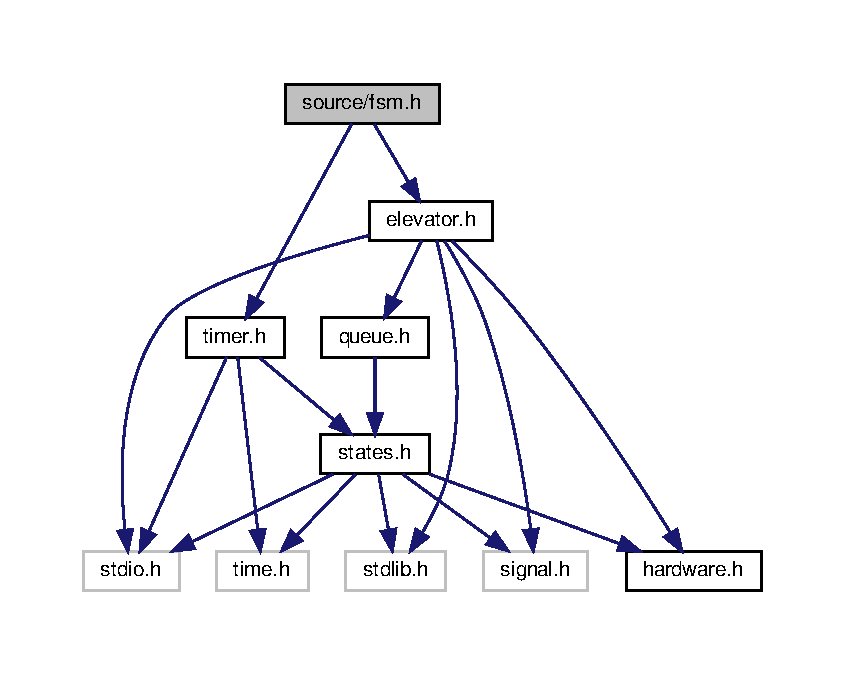
\includegraphics[width=350pt]{fsm_8h__incl}
\end{center}
\end{figure}
This graph shows which files directly or indirectly include this file\+:\nopagebreak
\begin{figure}[H]
\begin{center}
\leavevmode
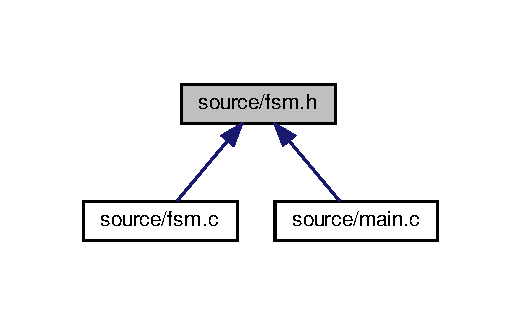
\includegraphics[width=250pt]{fsm_8h__dep__incl}
\end{center}
\end{figure}
\subsection*{Functions}
\begin{DoxyCompactItemize}
\item 
void \hyperlink{fsm_8h_a544184483e70276bdd08ea9387c759dc}{fsm\+\_\+init} (\hyperlink{structelevator}{elevator} $\ast$el)
\begin{DoxyCompactList}\small\item\em Initializes the elevator and moves it to a defined state. \end{DoxyCompactList}\item 
void \hyperlink{fsm_8h_a55b8638db8400e3a58de8a714900b88e}{fsm\+\_\+switch} (\hyperlink{structelevator}{elevator} $\ast$el)
\begin{DoxyCompactList}\small\item\em Loop that controls the elevator. Contains the logic for the finite state machine. \end{DoxyCompactList}\item 
void \hyperlink{fsm_8h_aac27fb6111ea92a93c516024ba4f96ef}{fsm\+\_\+idle} (\hyperlink{structelevator}{elevator} $\ast$el)
\begin{DoxyCompactList}\small\item\em Function called when the elevator is in state I\+D\+LE. If there is a request at current floor, enters state {\ttfamily D\+O\+O\+R\+\_\+\+O\+P\+EN}. Otherwise if there is a request above or below, enters state {\ttfamily M\+O\+VE}. \end{DoxyCompactList}\item 
void \hyperlink{fsm_8h_a5d1c77afef3d5331db952c4812d22a1f}{fsm\+\_\+move} (\hyperlink{structelevator}{elevator} $\ast$el)
\begin{DoxyCompactList}\small\item\em Function called when the elevator is in state M\+O\+VE. Sets direction and starts the motor. If the elevator should take order at current floor, enters state {\ttfamily I\+D\+LE}. \end{DoxyCompactList}\item 
void \hyperlink{fsm_8h_a9967fc494ad00be3ebde2163464c016f}{fsm\+\_\+door\+\_\+open} (\hyperlink{structelevator}{elevator} $\ast$el)
\begin{DoxyCompactList}\small\item\em Function called when the elevator is in state D\+O\+OR O\+P\+EN. Commands door open, starts the timer and checks for any obstructions. Closes the door when the time is up and clears excecuted orders. Then enters state {\ttfamily I\+D\+LE}. \end{DoxyCompactList}\item 
void \hyperlink{fsm_8h_a69c1174f8092050b76f11aa072901ce3}{fsm\+\_\+emergency\+\_\+stop} (\hyperlink{structelevator}{elevator} $\ast$el)
\begin{DoxyCompactList}\small\item\em Function called when the elevator is in state E\+M\+E\+R\+G\+E\+N\+CY S\+T\+OP. Stops the elevator and sets the stop light. Clears the queue. If the elevator is at a floor the door is opened and when the stop button is released the elevator enters state {\ttfamily D\+O\+O\+R\+\_\+\+O\+P\+EN}. Otherwise it awaits until any requests is made, and then enters {\ttfamily M\+O\+VE}. \end{DoxyCompactList}\end{DoxyCompactItemize}


\subsection{Detailed Description}
The finite state machine. 



\subsection{Function Documentation}
\mbox{\Hypertarget{fsm_8h_a9967fc494ad00be3ebde2163464c016f}\label{fsm_8h_a9967fc494ad00be3ebde2163464c016f}} 
\index{fsm.\+h@{fsm.\+h}!fsm\+\_\+door\+\_\+open@{fsm\+\_\+door\+\_\+open}}
\index{fsm\+\_\+door\+\_\+open@{fsm\+\_\+door\+\_\+open}!fsm.\+h@{fsm.\+h}}
\subsubsection{\texorpdfstring{fsm\+\_\+door\+\_\+open()}{fsm\_door\_open()}}
{\footnotesize\ttfamily void fsm\+\_\+door\+\_\+open (\begin{DoxyParamCaption}\item[{\hyperlink{structelevator}{elevator} $\ast$}]{el }\end{DoxyParamCaption})}



Function called when the elevator is in state D\+O\+OR O\+P\+EN. Commands door open, starts the timer and checks for any obstructions. Closes the door when the time is up and clears excecuted orders. Then enters state {\ttfamily I\+D\+LE}. 


\begin{DoxyParams}[1]{Parameters}
\mbox{\tt in,out}  & {\em el} & The elevator. \\
\hline
\end{DoxyParams}


Definition at line 79 of file fsm.\+c.

\mbox{\Hypertarget{fsm_8h_a69c1174f8092050b76f11aa072901ce3}\label{fsm_8h_a69c1174f8092050b76f11aa072901ce3}} 
\index{fsm.\+h@{fsm.\+h}!fsm\+\_\+emergency\+\_\+stop@{fsm\+\_\+emergency\+\_\+stop}}
\index{fsm\+\_\+emergency\+\_\+stop@{fsm\+\_\+emergency\+\_\+stop}!fsm.\+h@{fsm.\+h}}
\subsubsection{\texorpdfstring{fsm\+\_\+emergency\+\_\+stop()}{fsm\_emergency\_stop()}}
{\footnotesize\ttfamily void fsm\+\_\+emergency\+\_\+stop (\begin{DoxyParamCaption}\item[{\hyperlink{structelevator}{elevator} $\ast$}]{el }\end{DoxyParamCaption})}



Function called when the elevator is in state E\+M\+E\+R\+G\+E\+N\+CY S\+T\+OP. Stops the elevator and sets the stop light. Clears the queue. If the elevator is at a floor the door is opened and when the stop button is released the elevator enters state {\ttfamily D\+O\+O\+R\+\_\+\+O\+P\+EN}. Otherwise it awaits until any requests is made, and then enters {\ttfamily M\+O\+VE}. 


\begin{DoxyParams}[1]{Parameters}
\mbox{\tt in,out}  & {\em el} & The elevator. \\
\hline
\end{DoxyParams}


Definition at line 109 of file fsm.\+c.

\mbox{\Hypertarget{fsm_8h_aac27fb6111ea92a93c516024ba4f96ef}\label{fsm_8h_aac27fb6111ea92a93c516024ba4f96ef}} 
\index{fsm.\+h@{fsm.\+h}!fsm\+\_\+idle@{fsm\+\_\+idle}}
\index{fsm\+\_\+idle@{fsm\+\_\+idle}!fsm.\+h@{fsm.\+h}}
\subsubsection{\texorpdfstring{fsm\+\_\+idle()}{fsm\_idle()}}
{\footnotesize\ttfamily void fsm\+\_\+idle (\begin{DoxyParamCaption}\item[{\hyperlink{structelevator}{elevator} $\ast$}]{el }\end{DoxyParamCaption})}



Function called when the elevator is in state I\+D\+LE. If there is a request at current floor, enters state {\ttfamily D\+O\+O\+R\+\_\+\+O\+P\+EN}. Otherwise if there is a request above or below, enters state {\ttfamily M\+O\+VE}. 


\begin{DoxyParams}[1]{Parameters}
\mbox{\tt in,out}  & {\em el} & The elevator. \\
\hline
\end{DoxyParams}


Definition at line 53 of file fsm.\+c.

\mbox{\Hypertarget{fsm_8h_a544184483e70276bdd08ea9387c759dc}\label{fsm_8h_a544184483e70276bdd08ea9387c759dc}} 
\index{fsm.\+h@{fsm.\+h}!fsm\+\_\+init@{fsm\+\_\+init}}
\index{fsm\+\_\+init@{fsm\+\_\+init}!fsm.\+h@{fsm.\+h}}
\subsubsection{\texorpdfstring{fsm\+\_\+init()}{fsm\_init()}}
{\footnotesize\ttfamily void fsm\+\_\+init (\begin{DoxyParamCaption}\item[{\hyperlink{structelevator}{elevator} $\ast$}]{el }\end{DoxyParamCaption})}



Initializes the elevator and moves it to a defined state. 


\begin{DoxyParams}[1]{Parameters}
\mbox{\tt in,out}  & {\em el} & The elevator. \\
\hline
\end{DoxyParams}


Definition at line 3 of file fsm.\+c.

\mbox{\Hypertarget{fsm_8h_a5d1c77afef3d5331db952c4812d22a1f}\label{fsm_8h_a5d1c77afef3d5331db952c4812d22a1f}} 
\index{fsm.\+h@{fsm.\+h}!fsm\+\_\+move@{fsm\+\_\+move}}
\index{fsm\+\_\+move@{fsm\+\_\+move}!fsm.\+h@{fsm.\+h}}
\subsubsection{\texorpdfstring{fsm\+\_\+move()}{fsm\_move()}}
{\footnotesize\ttfamily void fsm\+\_\+move (\begin{DoxyParamCaption}\item[{\hyperlink{structelevator}{elevator} $\ast$}]{el }\end{DoxyParamCaption})}



Function called when the elevator is in state M\+O\+VE. Sets direction and starts the motor. If the elevator should take order at current floor, enters state {\ttfamily I\+D\+LE}. 


\begin{DoxyParams}[1]{Parameters}
\mbox{\tt in,out}  & {\em el} & The elevator. \\
\hline
\end{DoxyParams}


Definition at line 65 of file fsm.\+c.

\mbox{\Hypertarget{fsm_8h_a55b8638db8400e3a58de8a714900b88e}\label{fsm_8h_a55b8638db8400e3a58de8a714900b88e}} 
\index{fsm.\+h@{fsm.\+h}!fsm\+\_\+switch@{fsm\+\_\+switch}}
\index{fsm\+\_\+switch@{fsm\+\_\+switch}!fsm.\+h@{fsm.\+h}}
\subsubsection{\texorpdfstring{fsm\+\_\+switch()}{fsm\_switch()}}
{\footnotesize\ttfamily void fsm\+\_\+switch (\begin{DoxyParamCaption}\item[{\hyperlink{structelevator}{elevator} $\ast$}]{el }\end{DoxyParamCaption})}



Loop that controls the elevator. Contains the logic for the finite state machine. 


\begin{DoxyParams}[1]{Parameters}
\mbox{\tt in,out}  & {\em el} & The elevator. \\
\hline
\end{DoxyParams}


Definition at line 23 of file fsm.\+c.


\hypertarget{hardware_8h}{}\section{source/hardware.h File Reference}
\label{hardware_8h}\index{source/hardware.\+h@{source/hardware.\+h}}


Driver for the elevator hardware.  


This graph shows which files directly or indirectly include this file\+:\nopagebreak
\begin{figure}[H]
\begin{center}
\leavevmode
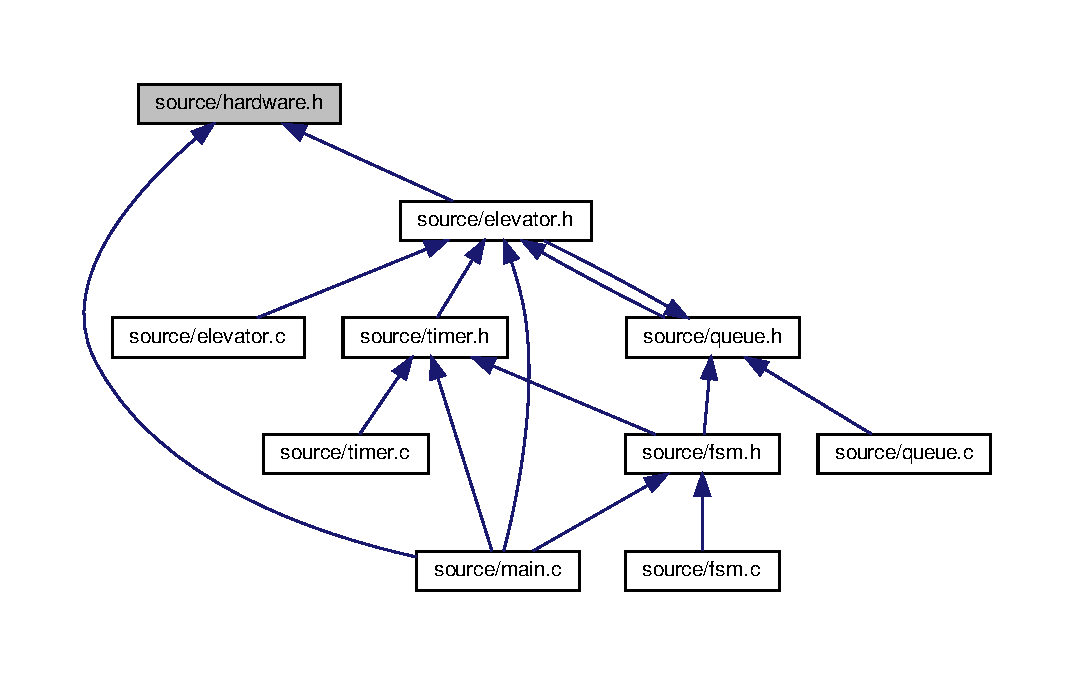
\includegraphics[width=350pt]{hardware_8h__dep__incl}
\end{center}
\end{figure}
\subsection*{Macros}
\begin{DoxyCompactItemize}
\item 
\mbox{\Hypertarget{hardware_8h_ae9e42615eade15633bd8c03b7a271a00}\label{hardware_8h_ae9e42615eade15633bd8c03b7a271a00}} 
\#define {\bfseries H\+A\+R\+D\+W\+A\+R\+E\+\_\+\+N\+U\+M\+B\+E\+R\+\_\+\+O\+F\+\_\+\+F\+L\+O\+O\+RS}~4
\item 
\mbox{\Hypertarget{hardware_8h_a966cbacea011640db5803364bff5ed53}\label{hardware_8h_a966cbacea011640db5803364bff5ed53}} 
\#define {\bfseries H\+A\+R\+D\+W\+A\+R\+E\+\_\+\+N\+U\+M\+B\+E\+R\+\_\+\+O\+F\+\_\+\+B\+U\+T\+T\+O\+NS}~3
\end{DoxyCompactItemize}
\subsection*{Enumerations}
\begin{DoxyCompactItemize}
\item 
\mbox{\Hypertarget{hardware_8h_a2167c399a24df296afc432bcb88228af}\label{hardware_8h_a2167c399a24df296afc432bcb88228af}} 
enum \hyperlink{hardware_8h_a2167c399a24df296afc432bcb88228af}{Hardware\+Movement} \{ {\bfseries H\+A\+R\+D\+W\+A\+R\+E\+\_\+\+M\+O\+V\+E\+M\+E\+N\+T\+\_\+\+UP}, 
{\bfseries H\+A\+R\+D\+W\+A\+R\+E\+\_\+\+M\+O\+V\+E\+M\+E\+N\+T\+\_\+\+S\+T\+OP}, 
{\bfseries H\+A\+R\+D\+W\+A\+R\+E\+\_\+\+M\+O\+V\+E\+M\+E\+N\+T\+\_\+\+D\+O\+WN}
 \}\begin{DoxyCompactList}\small\item\em Movement type used in {\ttfamily hardware\+\_\+command\+\_\+movement}. \end{DoxyCompactList}
\item 
\mbox{\Hypertarget{hardware_8h_a796a8de8ce0ae769d7dbd3327a7bdbe7}\label{hardware_8h_a796a8de8ce0ae769d7dbd3327a7bdbe7}} 
enum \hyperlink{hardware_8h_a796a8de8ce0ae769d7dbd3327a7bdbe7}{Hardware\+Order} \{ {\bfseries H\+A\+R\+D\+W\+A\+R\+E\+\_\+\+O\+R\+D\+E\+R\+\_\+\+UP}, 
{\bfseries H\+A\+R\+D\+W\+A\+R\+E\+\_\+\+O\+R\+D\+E\+R\+\_\+\+I\+N\+S\+I\+DE}, 
{\bfseries H\+A\+R\+D\+W\+A\+R\+E\+\_\+\+O\+R\+D\+E\+R\+\_\+\+D\+O\+WN}
 \}\begin{DoxyCompactList}\small\item\em Order type used in {\ttfamily hardware\+\_\+read\+\_\+order} and in {\ttfamily hardware\+\_\+command\+\_\+order\+\_\+light}. \end{DoxyCompactList}
\end{DoxyCompactItemize}
\subsection*{Functions}
\begin{DoxyCompactItemize}
\item 
int \hyperlink{hardware_8h_a054b8fb8768311d46be58d6a4890d771}{hardware\+\_\+init} ()
\begin{DoxyCompactList}\small\item\em Initializes the elevator control hardware. Must be called once before other calls to the elevator hardware driver. \end{DoxyCompactList}\item 
void \hyperlink{hardware_8h_a01de081ef0510a111053c18cd31afa27}{hardware\+\_\+command\+\_\+movement} (\hyperlink{hardware_8h_a2167c399a24df296afc432bcb88228af}{Hardware\+Movement} movement)
\begin{DoxyCompactList}\small\item\em Commands the elevator to either move up or down, or commands it to halt. \end{DoxyCompactList}\item 
int \hyperlink{hardware_8h_a4a77b27c86675c00b513db3445966804}{hardware\+\_\+read\+\_\+stop\+\_\+signal} ()
\begin{DoxyCompactList}\small\item\em Polls the hardware for the current stop signal. \end{DoxyCompactList}\item 
int \hyperlink{hardware_8h_a459fe57a3ee4bc2a28e8a15b2ab14c2d}{hardware\+\_\+read\+\_\+obstruction\+\_\+signal} ()
\begin{DoxyCompactList}\small\item\em Polls the hardware for the current obstruction signal. \end{DoxyCompactList}\item 
int \hyperlink{hardware_8h_ab048489e6302bb5604aad753f2d7d501}{hardware\+\_\+read\+\_\+floor\+\_\+sensor} (int floor)
\begin{DoxyCompactList}\small\item\em Polls the floor sensor for the given {\ttfamily floor}. \end{DoxyCompactList}\item 
int \hyperlink{hardware_8h_a87917f3aa093fb46ca821a400d011ee8}{hardware\+\_\+read\+\_\+order} (int floor, \hyperlink{hardware_8h_a796a8de8ce0ae769d7dbd3327a7bdbe7}{Hardware\+Order} order\+\_\+type)
\begin{DoxyCompactList}\small\item\em Polls the hardware for the status of orders from floor {\ttfamily floor} of type {\ttfamily order\+\_\+type}. \end{DoxyCompactList}\item 
void \hyperlink{hardware_8h_a80d99ddaa8e7b58c9a88b60ea553c1b6}{hardware\+\_\+command\+\_\+door\+\_\+open} (int door\+\_\+open)
\begin{DoxyCompactList}\small\item\em Commands the hardware to open-\/ or close the elevator door. \end{DoxyCompactList}\item 
void \hyperlink{hardware_8h_a407a6ec035ba357de6aa0fbe55501d1e}{hardware\+\_\+command\+\_\+floor\+\_\+indicator\+\_\+on} (int floor)
\begin{DoxyCompactList}\small\item\em Commands the hardware to turn on the floor indicator for {\ttfamily floor}. All indicators all mutually exclusive; other indicator lights will turn off. \end{DoxyCompactList}\item 
void \hyperlink{hardware_8h_aa75b3ac17f72b25946414f48d0063a10}{hardware\+\_\+command\+\_\+stop\+\_\+light} (int on)
\begin{DoxyCompactList}\small\item\em Sets the light in the panel stop button. \end{DoxyCompactList}\item 
void \hyperlink{hardware_8h_aa9b33faa52f0ec5b614d3e7dc05be140}{hardware\+\_\+command\+\_\+order\+\_\+light} (int floor, \hyperlink{hardware_8h_a796a8de8ce0ae769d7dbd3327a7bdbe7}{Hardware\+Order} order\+\_\+type, int on)
\begin{DoxyCompactList}\small\item\em Sets the light in a button corresponding to an order of type {\ttfamily order\+\_\+type}, at floor {\ttfamily floor}. \end{DoxyCompactList}\end{DoxyCompactItemize}


\subsection{Detailed Description}
Driver for the elevator hardware. 



\subsection{Function Documentation}
\mbox{\Hypertarget{hardware_8h_a80d99ddaa8e7b58c9a88b60ea553c1b6}\label{hardware_8h_a80d99ddaa8e7b58c9a88b60ea553c1b6}} 
\index{hardware.\+h@{hardware.\+h}!hardware\+\_\+command\+\_\+door\+\_\+open@{hardware\+\_\+command\+\_\+door\+\_\+open}}
\index{hardware\+\_\+command\+\_\+door\+\_\+open@{hardware\+\_\+command\+\_\+door\+\_\+open}!hardware.\+h@{hardware.\+h}}
\subsubsection{\texorpdfstring{hardware\+\_\+command\+\_\+door\+\_\+open()}{hardware\_command\_door\_open()}}
{\footnotesize\ttfamily void hardware\+\_\+command\+\_\+door\+\_\+open (\begin{DoxyParamCaption}\item[{int}]{door\+\_\+open }\end{DoxyParamCaption})}



Commands the hardware to open-\/ or close the elevator door. 


\begin{DoxyParams}{Parameters}
{\em door\+\_\+open} & A truthy value (non-\/zero) to open the door; 0 to close. \\
\hline
\end{DoxyParams}


Definition at line 139 of file hardware\+\_\+sal.\+c.

\mbox{\Hypertarget{hardware_8h_a407a6ec035ba357de6aa0fbe55501d1e}\label{hardware_8h_a407a6ec035ba357de6aa0fbe55501d1e}} 
\index{hardware.\+h@{hardware.\+h}!hardware\+\_\+command\+\_\+floor\+\_\+indicator\+\_\+on@{hardware\+\_\+command\+\_\+floor\+\_\+indicator\+\_\+on}}
\index{hardware\+\_\+command\+\_\+floor\+\_\+indicator\+\_\+on@{hardware\+\_\+command\+\_\+floor\+\_\+indicator\+\_\+on}!hardware.\+h@{hardware.\+h}}
\subsubsection{\texorpdfstring{hardware\+\_\+command\+\_\+floor\+\_\+indicator\+\_\+on()}{hardware\_command\_floor\_indicator\_on()}}
{\footnotesize\ttfamily void hardware\+\_\+command\+\_\+floor\+\_\+indicator\+\_\+on (\begin{DoxyParamCaption}\item[{int}]{floor }\end{DoxyParamCaption})}



Commands the hardware to turn on the floor indicator for {\ttfamily floor}. All indicators all mutually exclusive; other indicator lights will turn off. 


\begin{DoxyParams}{Parameters}
{\em floor} & Floor to turn on the indicator for.\\
\hline
\end{DoxyParams}
\begin{DoxyWarning}{Warning}
Owing to peculiarities in the hardware construction, there will always be one indicator active. 
\end{DoxyWarning}


Definition at line 148 of file hardware\+\_\+sal.\+c.

\mbox{\Hypertarget{hardware_8h_a01de081ef0510a111053c18cd31afa27}\label{hardware_8h_a01de081ef0510a111053c18cd31afa27}} 
\index{hardware.\+h@{hardware.\+h}!hardware\+\_\+command\+\_\+movement@{hardware\+\_\+command\+\_\+movement}}
\index{hardware\+\_\+command\+\_\+movement@{hardware\+\_\+command\+\_\+movement}!hardware.\+h@{hardware.\+h}}
\subsubsection{\texorpdfstring{hardware\+\_\+command\+\_\+movement()}{hardware\_command\_movement()}}
{\footnotesize\ttfamily void hardware\+\_\+command\+\_\+movement (\begin{DoxyParamCaption}\item[{\hyperlink{hardware_8h_a2167c399a24df296afc432bcb88228af}{Hardware\+Movement}}]{movement }\end{DoxyParamCaption})}



Commands the elevator to either move up or down, or commands it to halt. 


\begin{DoxyParams}{Parameters}
{\em movement} & Commanded movement. \\
\hline
\end{DoxyParams}


Definition at line 70 of file hardware\+\_\+sal.\+c.

\mbox{\Hypertarget{hardware_8h_aa9b33faa52f0ec5b614d3e7dc05be140}\label{hardware_8h_aa9b33faa52f0ec5b614d3e7dc05be140}} 
\index{hardware.\+h@{hardware.\+h}!hardware\+\_\+command\+\_\+order\+\_\+light@{hardware\+\_\+command\+\_\+order\+\_\+light}}
\index{hardware\+\_\+command\+\_\+order\+\_\+light@{hardware\+\_\+command\+\_\+order\+\_\+light}!hardware.\+h@{hardware.\+h}}
\subsubsection{\texorpdfstring{hardware\+\_\+command\+\_\+order\+\_\+light()}{hardware\_command\_order\_light()}}
{\footnotesize\ttfamily void hardware\+\_\+command\+\_\+order\+\_\+light (\begin{DoxyParamCaption}\item[{int}]{floor,  }\item[{\hyperlink{hardware_8h_a796a8de8ce0ae769d7dbd3327a7bdbe7}{Hardware\+Order}}]{order\+\_\+type,  }\item[{int}]{on }\end{DoxyParamCaption})}



Sets the light in a button corresponding to an order of type {\ttfamily order\+\_\+type}, at floor {\ttfamily floor}. 


\begin{DoxyParams}{Parameters}
{\em floor} & The floor of the order indicator. \\
\hline
{\em order\+\_\+type} & The type of order. \\
\hline
{\em on} & A truthy value (non-\/zero) to turn the light on; 0 to turn it off. \\
\hline
\end{DoxyParams}


Definition at line 173 of file hardware\+\_\+sal.\+c.

\mbox{\Hypertarget{hardware_8h_aa75b3ac17f72b25946414f48d0063a10}\label{hardware_8h_aa75b3ac17f72b25946414f48d0063a10}} 
\index{hardware.\+h@{hardware.\+h}!hardware\+\_\+command\+\_\+stop\+\_\+light@{hardware\+\_\+command\+\_\+stop\+\_\+light}}
\index{hardware\+\_\+command\+\_\+stop\+\_\+light@{hardware\+\_\+command\+\_\+stop\+\_\+light}!hardware.\+h@{hardware.\+h}}
\subsubsection{\texorpdfstring{hardware\+\_\+command\+\_\+stop\+\_\+light()}{hardware\_command\_stop\_light()}}
{\footnotesize\ttfamily void hardware\+\_\+command\+\_\+stop\+\_\+light (\begin{DoxyParamCaption}\item[{int}]{on }\end{DoxyParamCaption})}



Sets the light in the panel stop button. 


\begin{DoxyParams}{Parameters}
{\em on} & A truthy value (non-\/zero) to turn the light on; 0 to turn it off. \\
\hline
\end{DoxyParams}


Definition at line 164 of file hardware\+\_\+sal.\+c.

\mbox{\Hypertarget{hardware_8h_a054b8fb8768311d46be58d6a4890d771}\label{hardware_8h_a054b8fb8768311d46be58d6a4890d771}} 
\index{hardware.\+h@{hardware.\+h}!hardware\+\_\+init@{hardware\+\_\+init}}
\index{hardware\+\_\+init@{hardware\+\_\+init}!hardware.\+h@{hardware.\+h}}
\subsubsection{\texorpdfstring{hardware\+\_\+init()}{hardware\_init()}}
{\footnotesize\ttfamily int hardware\+\_\+init (\begin{DoxyParamCaption}{ }\end{DoxyParamCaption})}



Initializes the elevator control hardware. Must be called once before other calls to the elevator hardware driver. 

\begin{DoxyReturn}{Returns}
0 on success. Non-\/zero for failure. 
\end{DoxyReturn}


Definition at line 46 of file hardware\+\_\+sal.\+c.

\mbox{\Hypertarget{hardware_8h_ab048489e6302bb5604aad753f2d7d501}\label{hardware_8h_ab048489e6302bb5604aad753f2d7d501}} 
\index{hardware.\+h@{hardware.\+h}!hardware\+\_\+read\+\_\+floor\+\_\+sensor@{hardware\+\_\+read\+\_\+floor\+\_\+sensor}}
\index{hardware\+\_\+read\+\_\+floor\+\_\+sensor@{hardware\+\_\+read\+\_\+floor\+\_\+sensor}!hardware.\+h@{hardware.\+h}}
\subsubsection{\texorpdfstring{hardware\+\_\+read\+\_\+floor\+\_\+sensor()}{hardware\_read\_floor\_sensor()}}
{\footnotesize\ttfamily int hardware\+\_\+read\+\_\+floor\+\_\+sensor (\begin{DoxyParamCaption}\item[{int}]{floor }\end{DoxyParamCaption})}



Polls the floor sensor for the given {\ttfamily floor}. 


\begin{DoxyParams}{Parameters}
{\em floor} & Inquired floor.\\
\hline
\end{DoxyParams}
\begin{DoxyReturn}{Returns}
1 if the elevator is at {\ttfamily floor}, otherwise 0; 
\end{DoxyReturn}


Definition at line 96 of file hardware\+\_\+sal.\+c.

\mbox{\Hypertarget{hardware_8h_a459fe57a3ee4bc2a28e8a15b2ab14c2d}\label{hardware_8h_a459fe57a3ee4bc2a28e8a15b2ab14c2d}} 
\index{hardware.\+h@{hardware.\+h}!hardware\+\_\+read\+\_\+obstruction\+\_\+signal@{hardware\+\_\+read\+\_\+obstruction\+\_\+signal}}
\index{hardware\+\_\+read\+\_\+obstruction\+\_\+signal@{hardware\+\_\+read\+\_\+obstruction\+\_\+signal}!hardware.\+h@{hardware.\+h}}
\subsubsection{\texorpdfstring{hardware\+\_\+read\+\_\+obstruction\+\_\+signal()}{hardware\_read\_obstruction\_signal()}}
{\footnotesize\ttfamily int hardware\+\_\+read\+\_\+obstruction\+\_\+signal (\begin{DoxyParamCaption}{ }\end{DoxyParamCaption})}



Polls the hardware for the current obstruction signal. 

\begin{DoxyReturn}{Returns}
1 if the obstruction signal is high; 0 if it is low. 
\end{DoxyReturn}


Definition at line 92 of file hardware\+\_\+sal.\+c.

\mbox{\Hypertarget{hardware_8h_a87917f3aa093fb46ca821a400d011ee8}\label{hardware_8h_a87917f3aa093fb46ca821a400d011ee8}} 
\index{hardware.\+h@{hardware.\+h}!hardware\+\_\+read\+\_\+order@{hardware\+\_\+read\+\_\+order}}
\index{hardware\+\_\+read\+\_\+order@{hardware\+\_\+read\+\_\+order}!hardware.\+h@{hardware.\+h}}
\subsubsection{\texorpdfstring{hardware\+\_\+read\+\_\+order()}{hardware\_read\_order()}}
{\footnotesize\ttfamily int hardware\+\_\+read\+\_\+order (\begin{DoxyParamCaption}\item[{int}]{floor,  }\item[{\hyperlink{hardware_8h_a796a8de8ce0ae769d7dbd3327a7bdbe7}{Hardware\+Order}}]{order\+\_\+type }\end{DoxyParamCaption})}



Polls the hardware for the status of orders from floor {\ttfamily floor} of type {\ttfamily order\+\_\+type}. 


\begin{DoxyParams}{Parameters}
{\em floor} & Inquired floor. \\
\hline
{\em order\+\_\+type} & \\
\hline
\end{DoxyParams}
\begin{DoxyReturn}{Returns}
1 if the combination of {\ttfamily floor} and {\ttfamily order\+\_\+type} is being requested, otherwise 0. 
\end{DoxyReturn}


Definition at line 122 of file hardware\+\_\+sal.\+c.

\mbox{\Hypertarget{hardware_8h_a4a77b27c86675c00b513db3445966804}\label{hardware_8h_a4a77b27c86675c00b513db3445966804}} 
\index{hardware.\+h@{hardware.\+h}!hardware\+\_\+read\+\_\+stop\+\_\+signal@{hardware\+\_\+read\+\_\+stop\+\_\+signal}}
\index{hardware\+\_\+read\+\_\+stop\+\_\+signal@{hardware\+\_\+read\+\_\+stop\+\_\+signal}!hardware.\+h@{hardware.\+h}}
\subsubsection{\texorpdfstring{hardware\+\_\+read\+\_\+stop\+\_\+signal()}{hardware\_read\_stop\_signal()}}
{\footnotesize\ttfamily int hardware\+\_\+read\+\_\+stop\+\_\+signal (\begin{DoxyParamCaption}{ }\end{DoxyParamCaption})}



Polls the hardware for the current stop signal. 

\begin{DoxyReturn}{Returns}
1 if the stop signal is high; 0 if it is low. 
\end{DoxyReturn}


Definition at line 88 of file hardware\+\_\+sal.\+c.


\hypertarget{queue_8h}{}\section{source/queue.h File Reference}
\label{queue_8h}\index{source/queue.\+h@{source/queue.\+h}}


Takes care of the elevator\textquotesingle{}s queue.  


{\ttfamily \#include \char`\"{}states.\+h\char`\"{}}\newline
Include dependency graph for queue.\+h\+:\nopagebreak
\begin{figure}[H]
\begin{center}
\leavevmode
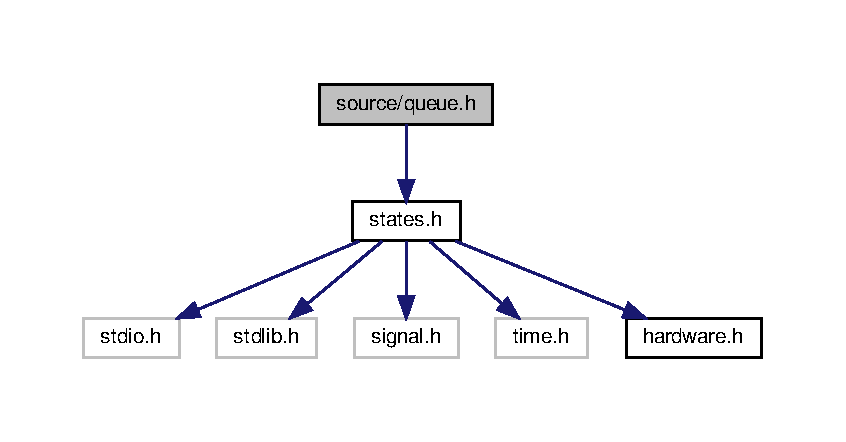
\includegraphics[width=350pt]{queue_8h__incl}
\end{center}
\end{figure}
This graph shows which files directly or indirectly include this file\+:\nopagebreak
\begin{figure}[H]
\begin{center}
\leavevmode
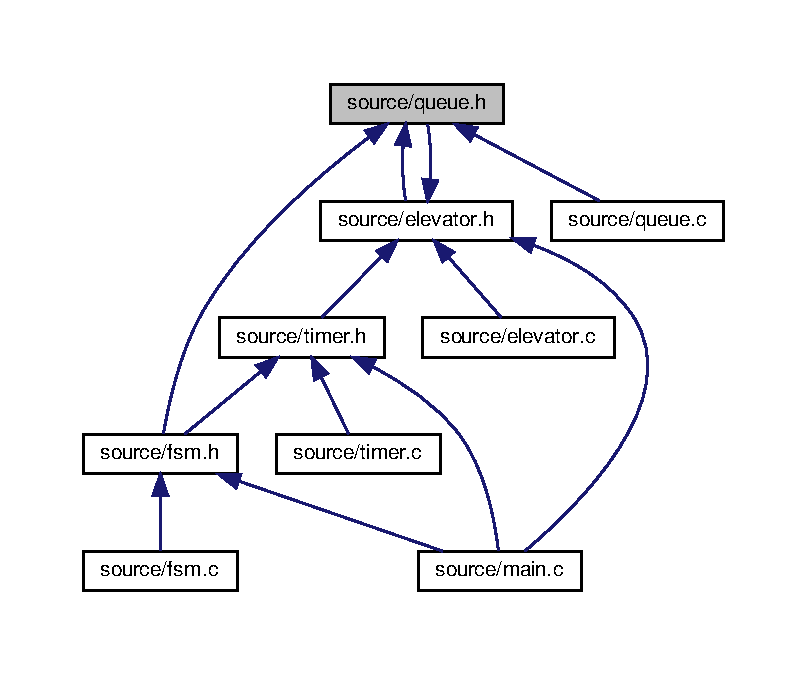
\includegraphics[width=324pt]{queue_8h__dep__incl}
\end{center}
\end{figure}
\subsection*{Functions}
\begin{DoxyCompactItemize}
\item 
void \hyperlink{queue_8h_ab71868b345d53175364434fd5c0dc0bf}{queue\+\_\+update} (\hyperlink{structelevator}{elevator} $\ast$el)
\begin{DoxyCompactList}\small\item\em Updates the queue with new orders. \end{DoxyCompactList}\item 
void \hyperlink{queue_8h_a236ea41418c66779dc0ce6ac2709e9af}{queue\+\_\+clear\+\_\+all} (\hyperlink{structelevator}{elevator} $\ast$el)
\begin{DoxyCompactList}\small\item\em Clears all orders (0). Unavaliable orders are given the value -\/1. \end{DoxyCompactList}\item 
int \hyperlink{queue_8h_a5f57d47d6d4c79d5f79d86d2e637b6a7}{queue\+\_\+orders\+\_\+at\+\_\+floor} (\hyperlink{structelevator}{elevator} $\ast$el)
\begin{DoxyCompactList}\small\item\em Checks if the queue contains any orders at its current floor. \end{DoxyCompactList}\item 
int \hyperlink{queue_8h_a2b04fb0831b618d272657b6bd783f723}{queue\+\_\+orders\+\_\+above} (\hyperlink{structelevator}{elevator} $\ast$el)
\begin{DoxyCompactList}\small\item\em Checks if the queue contains any orders above its current floor. \end{DoxyCompactList}\item 
int \hyperlink{queue_8h_afc97a824f1fae7d8a5aca0d74c261b79}{queue\+\_\+orders\+\_\+below} (\hyperlink{structelevator}{elevator} $\ast$el)
\begin{DoxyCompactList}\small\item\em Checks if the queue contains any orders below its current floor. \end{DoxyCompactList}\item 
int \hyperlink{queue_8h_afc4f556ab3ec5b6a722d14f951234f8f}{queue\+\_\+take\+\_\+order} (\hyperlink{structelevator}{elevator} $\ast$el)
\begin{DoxyCompactList}\small\item\em Checks if the elevator should take the order at current floor. \end{DoxyCompactList}\item 
void \hyperlink{queue_8h_abc88f9451cea49981f06706b45780b55}{queue\+\_\+clear\+\_\+executed\+\_\+order} (\hyperlink{structelevator}{elevator} $\ast$el)
\begin{DoxyCompactList}\small\item\em Deletes executed orders at current floor. \end{DoxyCompactList}\item 
void \hyperlink{queue_8h_a9790c01f8f7731447328bd65b393dc4e}{queue\+\_\+set\+\_\+light} (\hyperlink{structelevator}{elevator} $\ast$el)
\begin{DoxyCompactList}\small\item\em Sets the order lights of the buttons that have been pulled. \end{DoxyCompactList}\item 
void \hyperlink{queue_8h_a67c922a64bce6216dddc3ccca0e1eb43}{queue\+\_\+clear\+\_\+light} (\hyperlink{structelevator}{elevator} $\ast$el)
\begin{DoxyCompactList}\small\item\em Clears the order lights for executed orders. \end{DoxyCompactList}\item 
void \hyperlink{queue_8h_ae3498650822c7f05e23cf2c62f6cc212}{queue\+\_\+clear\+\_\+all\+\_\+lights} (\hyperlink{structelevator}{elevator} $\ast$el)
\begin{DoxyCompactList}\small\item\em Clears all order lights. \end{DoxyCompactList}\item 
void \hyperlink{queue_8h_a023bd49134ae52c1e2c1252d731c4fb0}{queue\+\_\+print} (\hyperlink{structelevator}{elevator} $\ast$el)
\begin{DoxyCompactList}\small\item\em Prints the queue as a matrix. \end{DoxyCompactList}\end{DoxyCompactItemize}


\subsection{Detailed Description}
Takes care of the elevator\textquotesingle{}s queue. 



\subsection{Function Documentation}
\mbox{\Hypertarget{queue_8h_a236ea41418c66779dc0ce6ac2709e9af}\label{queue_8h_a236ea41418c66779dc0ce6ac2709e9af}} 
\index{queue.\+h@{queue.\+h}!queue\+\_\+clear\+\_\+all@{queue\+\_\+clear\+\_\+all}}
\index{queue\+\_\+clear\+\_\+all@{queue\+\_\+clear\+\_\+all}!queue.\+h@{queue.\+h}}
\subsubsection{\texorpdfstring{queue\+\_\+clear\+\_\+all()}{queue\_clear\_all()}}
{\footnotesize\ttfamily void queue\+\_\+clear\+\_\+all (\begin{DoxyParamCaption}\item[{\hyperlink{structelevator}{elevator} $\ast$}]{el }\end{DoxyParamCaption})}



Clears all orders (0). Unavaliable orders are given the value -\/1. 


\begin{DoxyParams}[1]{Parameters}
\mbox{\tt in,out}  & {\em el} & The elevator. \\
\hline
\end{DoxyParams}


Definition at line 16 of file queue.\+c.

\mbox{\Hypertarget{queue_8h_ae3498650822c7f05e23cf2c62f6cc212}\label{queue_8h_ae3498650822c7f05e23cf2c62f6cc212}} 
\index{queue.\+h@{queue.\+h}!queue\+\_\+clear\+\_\+all\+\_\+lights@{queue\+\_\+clear\+\_\+all\+\_\+lights}}
\index{queue\+\_\+clear\+\_\+all\+\_\+lights@{queue\+\_\+clear\+\_\+all\+\_\+lights}!queue.\+h@{queue.\+h}}
\subsubsection{\texorpdfstring{queue\+\_\+clear\+\_\+all\+\_\+lights()}{queue\_clear\_all\_lights()}}
{\footnotesize\ttfamily void queue\+\_\+clear\+\_\+all\+\_\+lights (\begin{DoxyParamCaption}\item[{\hyperlink{structelevator}{elevator} $\ast$}]{el }\end{DoxyParamCaption})}



Clears all order lights. 


\begin{DoxyParams}[1]{Parameters}
\mbox{\tt in,out}  & {\em el} & The elevator. \\
\hline
\end{DoxyParams}


Definition at line 113 of file queue.\+c.

\mbox{\Hypertarget{queue_8h_abc88f9451cea49981f06706b45780b55}\label{queue_8h_abc88f9451cea49981f06706b45780b55}} 
\index{queue.\+h@{queue.\+h}!queue\+\_\+clear\+\_\+executed\+\_\+order@{queue\+\_\+clear\+\_\+executed\+\_\+order}}
\index{queue\+\_\+clear\+\_\+executed\+\_\+order@{queue\+\_\+clear\+\_\+executed\+\_\+order}!queue.\+h@{queue.\+h}}
\subsubsection{\texorpdfstring{queue\+\_\+clear\+\_\+executed\+\_\+order()}{queue\_clear\_executed\_order()}}
{\footnotesize\ttfamily void queue\+\_\+clear\+\_\+executed\+\_\+order (\begin{DoxyParamCaption}\item[{\hyperlink{structelevator}{elevator} $\ast$}]{el }\end{DoxyParamCaption})}



Deletes executed orders at current floor. 


\begin{DoxyParams}[1]{Parameters}
\mbox{\tt in,out}  & {\em el} & The elevator. \\
\hline
\end{DoxyParams}


Definition at line 83 of file queue.\+c.

\mbox{\Hypertarget{queue_8h_a67c922a64bce6216dddc3ccca0e1eb43}\label{queue_8h_a67c922a64bce6216dddc3ccca0e1eb43}} 
\index{queue.\+h@{queue.\+h}!queue\+\_\+clear\+\_\+light@{queue\+\_\+clear\+\_\+light}}
\index{queue\+\_\+clear\+\_\+light@{queue\+\_\+clear\+\_\+light}!queue.\+h@{queue.\+h}}
\subsubsection{\texorpdfstring{queue\+\_\+clear\+\_\+light()}{queue\_clear\_light()}}
{\footnotesize\ttfamily void queue\+\_\+clear\+\_\+light (\begin{DoxyParamCaption}\item[{\hyperlink{structelevator}{elevator} $\ast$}]{el }\end{DoxyParamCaption})}



Clears the order lights for executed orders. 


\begin{DoxyParams}[1]{Parameters}
\mbox{\tt in,out}  & {\em el} & The elevator. \\
\hline
\end{DoxyParams}


Definition at line 103 of file queue.\+c.

\mbox{\Hypertarget{queue_8h_a2b04fb0831b618d272657b6bd783f723}\label{queue_8h_a2b04fb0831b618d272657b6bd783f723}} 
\index{queue.\+h@{queue.\+h}!queue\+\_\+orders\+\_\+above@{queue\+\_\+orders\+\_\+above}}
\index{queue\+\_\+orders\+\_\+above@{queue\+\_\+orders\+\_\+above}!queue.\+h@{queue.\+h}}
\subsubsection{\texorpdfstring{queue\+\_\+orders\+\_\+above()}{queue\_orders\_above()}}
{\footnotesize\ttfamily int queue\+\_\+orders\+\_\+above (\begin{DoxyParamCaption}\item[{\hyperlink{structelevator}{elevator} $\ast$}]{el }\end{DoxyParamCaption})}



Checks if the queue contains any orders above its current floor. 


\begin{DoxyParams}[1]{Parameters}
\mbox{\tt in}  & {\em el} & The elevator. \\
\hline
\end{DoxyParams}
\begin{DoxyReturn}{Returns}
1 for success, 0 for failure. 
\end{DoxyReturn}


Definition at line 36 of file queue.\+c.

\mbox{\Hypertarget{queue_8h_a5f57d47d6d4c79d5f79d86d2e637b6a7}\label{queue_8h_a5f57d47d6d4c79d5f79d86d2e637b6a7}} 
\index{queue.\+h@{queue.\+h}!queue\+\_\+orders\+\_\+at\+\_\+floor@{queue\+\_\+orders\+\_\+at\+\_\+floor}}
\index{queue\+\_\+orders\+\_\+at\+\_\+floor@{queue\+\_\+orders\+\_\+at\+\_\+floor}!queue.\+h@{queue.\+h}}
\subsubsection{\texorpdfstring{queue\+\_\+orders\+\_\+at\+\_\+floor()}{queue\_orders\_at\_floor()}}
{\footnotesize\ttfamily int queue\+\_\+orders\+\_\+at\+\_\+floor (\begin{DoxyParamCaption}\item[{\hyperlink{structelevator}{elevator} $\ast$}]{el }\end{DoxyParamCaption})}



Checks if the queue contains any orders at its current floor. 


\begin{DoxyParams}[1]{Parameters}
\mbox{\tt in}  & {\em el} & The elevator. \\
\hline
\end{DoxyParams}
\begin{DoxyReturn}{Returns}
1 for success, 0 for failure. 
\end{DoxyReturn}


Definition at line 27 of file queue.\+c.

\mbox{\Hypertarget{queue_8h_afc97a824f1fae7d8a5aca0d74c261b79}\label{queue_8h_afc97a824f1fae7d8a5aca0d74c261b79}} 
\index{queue.\+h@{queue.\+h}!queue\+\_\+orders\+\_\+below@{queue\+\_\+orders\+\_\+below}}
\index{queue\+\_\+orders\+\_\+below@{queue\+\_\+orders\+\_\+below}!queue.\+h@{queue.\+h}}
\subsubsection{\texorpdfstring{queue\+\_\+orders\+\_\+below()}{queue\_orders\_below()}}
{\footnotesize\ttfamily int queue\+\_\+orders\+\_\+below (\begin{DoxyParamCaption}\item[{\hyperlink{structelevator}{elevator} $\ast$}]{el }\end{DoxyParamCaption})}



Checks if the queue contains any orders below its current floor. 


\begin{DoxyParams}[1]{Parameters}
\mbox{\tt in}  & {\em el} & The elevator. \\
\hline
\end{DoxyParams}
\begin{DoxyReturn}{Returns}
1 for success, 0 for failure. 
\end{DoxyReturn}


Definition at line 47 of file queue.\+c.

\mbox{\Hypertarget{queue_8h_a023bd49134ae52c1e2c1252d731c4fb0}\label{queue_8h_a023bd49134ae52c1e2c1252d731c4fb0}} 
\index{queue.\+h@{queue.\+h}!queue\+\_\+print@{queue\+\_\+print}}
\index{queue\+\_\+print@{queue\+\_\+print}!queue.\+h@{queue.\+h}}
\subsubsection{\texorpdfstring{queue\+\_\+print()}{queue\_print()}}
{\footnotesize\ttfamily void queue\+\_\+print (\begin{DoxyParamCaption}\item[{\hyperlink{structelevator}{elevator} $\ast$}]{el }\end{DoxyParamCaption})}



Prints the queue as a matrix. 


\begin{DoxyParams}[1]{Parameters}
\mbox{\tt in}  & {\em el} & The elevator. \\
\hline
\end{DoxyParams}


Definition at line 128 of file queue.\+c.

\mbox{\Hypertarget{queue_8h_a9790c01f8f7731447328bd65b393dc4e}\label{queue_8h_a9790c01f8f7731447328bd65b393dc4e}} 
\index{queue.\+h@{queue.\+h}!queue\+\_\+set\+\_\+light@{queue\+\_\+set\+\_\+light}}
\index{queue\+\_\+set\+\_\+light@{queue\+\_\+set\+\_\+light}!queue.\+h@{queue.\+h}}
\subsubsection{\texorpdfstring{queue\+\_\+set\+\_\+light()}{queue\_set\_light()}}
{\footnotesize\ttfamily void queue\+\_\+set\+\_\+light (\begin{DoxyParamCaption}\item[{\hyperlink{structelevator}{elevator} $\ast$}]{el }\end{DoxyParamCaption})}



Sets the order lights of the buttons that have been pulled. 


\begin{DoxyParams}[1]{Parameters}
\mbox{\tt in,out}  & {\em el} & The elevator. \\
\hline
\end{DoxyParams}


Definition at line 93 of file queue.\+c.

\mbox{\Hypertarget{queue_8h_afc4f556ab3ec5b6a722d14f951234f8f}\label{queue_8h_afc4f556ab3ec5b6a722d14f951234f8f}} 
\index{queue.\+h@{queue.\+h}!queue\+\_\+take\+\_\+order@{queue\+\_\+take\+\_\+order}}
\index{queue\+\_\+take\+\_\+order@{queue\+\_\+take\+\_\+order}!queue.\+h@{queue.\+h}}
\subsubsection{\texorpdfstring{queue\+\_\+take\+\_\+order()}{queue\_take\_order()}}
{\footnotesize\ttfamily int queue\+\_\+take\+\_\+order (\begin{DoxyParamCaption}\item[{\hyperlink{structelevator}{elevator} $\ast$}]{el }\end{DoxyParamCaption})}



Checks if the elevator should take the order at current floor. 


\begin{DoxyParams}[1]{Parameters}
\mbox{\tt in,out}  & {\em el} & The elevator. \\
\hline
\end{DoxyParams}
\begin{DoxyReturn}{Returns}
1 for success, 0 for failure. 
\end{DoxyReturn}


Definition at line 58 of file queue.\+c.

\mbox{\Hypertarget{queue_8h_ab71868b345d53175364434fd5c0dc0bf}\label{queue_8h_ab71868b345d53175364434fd5c0dc0bf}} 
\index{queue.\+h@{queue.\+h}!queue\+\_\+update@{queue\+\_\+update}}
\index{queue\+\_\+update@{queue\+\_\+update}!queue.\+h@{queue.\+h}}
\subsubsection{\texorpdfstring{queue\+\_\+update()}{queue\_update()}}
{\footnotesize\ttfamily void queue\+\_\+update (\begin{DoxyParamCaption}\item[{\hyperlink{structelevator}{elevator} $\ast$}]{el }\end{DoxyParamCaption})}



Updates the queue with new orders. 


\begin{DoxyParams}[1]{Parameters}
\mbox{\tt in,out}  & {\em el} & The elevator. \\
\hline
\end{DoxyParams}


Definition at line 3 of file queue.\+c.


\hypertarget{states_8h}{}\section{source/states.h File Reference}
\label{states_8h}\index{source/states.\+h@{source/states.\+h}}


Creates a struct for the elevator and an enumerator for its different states.  


{\ttfamily \#include $<$stdio.\+h$>$}\newline
{\ttfamily \#include $<$stdlib.\+h$>$}\newline
{\ttfamily \#include $<$signal.\+h$>$}\newline
{\ttfamily \#include $<$time.\+h$>$}\newline
{\ttfamily \#include \char`\"{}hardware.\+h\char`\"{}}\newline
Include dependency graph for states.\+h\+:\nopagebreak
\begin{figure}[H]
\begin{center}
\leavevmode
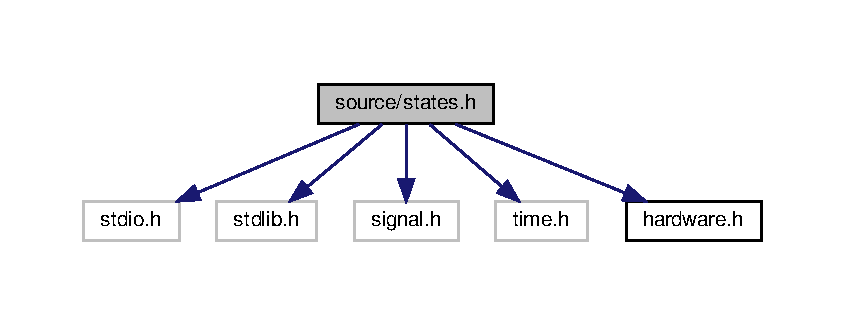
\includegraphics[width=350pt]{states_8h__incl}
\end{center}
\end{figure}
This graph shows which files directly or indirectly include this file\+:\nopagebreak
\begin{figure}[H]
\begin{center}
\leavevmode
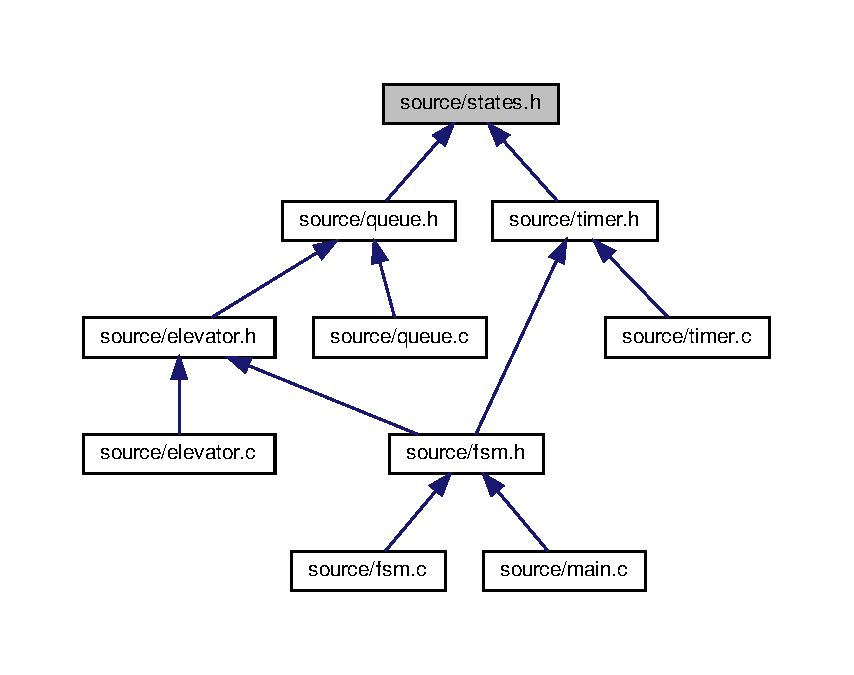
\includegraphics[width=350pt]{states_8h__dep__incl}
\end{center}
\end{figure}
\subsection*{Data Structures}
\begin{DoxyCompactItemize}
\item 
struct \hyperlink{structelevator}{elevator}
\begin{DoxyCompactList}\small\item\em A structure to represent the elevator. Contains memory of current state, queue of orders and time, as well as current and previous floor and direction. \end{DoxyCompactList}\end{DoxyCompactItemize}
\subsection*{Typedefs}
\begin{DoxyCompactItemize}
\item 
\mbox{\Hypertarget{states_8h_a5283e184f4663a2fd4c40e49f67bb794}\label{states_8h_a5283e184f4663a2fd4c40e49f67bb794}} 
typedef enum \hyperlink{states_8h_a09fd0473240586cf26c56b9c75589073}{elev\+\_\+state} \hyperlink{states_8h_a5283e184f4663a2fd4c40e49f67bb794}{elev\+\_\+state}
\begin{DoxyCompactList}\small\item\em The elevators different states. {\ttfamily I\+D\+LE}, {\ttfamily M\+O\+VE}, {\ttfamily D\+O\+O\+R\+\_\+\+O\+P\+EN}, {\ttfamily E\+M\+E\+R\+G\+E\+N\+C\+Y\+\_\+\+S\+T\+OP}. \end{DoxyCompactList}\item 
\mbox{\Hypertarget{states_8h_af6825629c9d12ceba0fcb13e3785378c}\label{states_8h_af6825629c9d12ceba0fcb13e3785378c}} 
typedef struct \hyperlink{structelevator}{elevator} \hyperlink{states_8h_af6825629c9d12ceba0fcb13e3785378c}{elevator}
\begin{DoxyCompactList}\small\item\em A structure to represent the elevator. Contains memory of current state, queue of orders and time, as well as current and previous floor and direction. \end{DoxyCompactList}\end{DoxyCompactItemize}
\subsection*{Enumerations}
\begin{DoxyCompactItemize}
\item 
\mbox{\Hypertarget{states_8h_a09fd0473240586cf26c56b9c75589073}\label{states_8h_a09fd0473240586cf26c56b9c75589073}} 
enum \hyperlink{states_8h_a09fd0473240586cf26c56b9c75589073}{elev\+\_\+state} \{ {\bfseries I\+D\+LE}, 
{\bfseries M\+O\+VE}, 
{\bfseries D\+O\+O\+R\+\_\+\+O\+P\+EN}, 
{\bfseries E\+M\+E\+R\+G\+E\+N\+C\+Y\+\_\+\+S\+T\+OP}
 \}\begin{DoxyCompactList}\small\item\em The elevators different states. {\ttfamily I\+D\+LE}, {\ttfamily M\+O\+VE}, {\ttfamily D\+O\+O\+R\+\_\+\+O\+P\+EN}, {\ttfamily E\+M\+E\+R\+G\+E\+N\+C\+Y\+\_\+\+S\+T\+OP}. \end{DoxyCompactList}
\end{DoxyCompactItemize}


\subsection{Detailed Description}
Creates a struct for the elevator and an enumerator for its different states. 


\hypertarget{timer_8h}{}\section{source/timer.h File Reference}
\label{timer_8h}\index{source/timer.\+h@{source/timer.\+h}}


Functions to keep the door open for a period of time.  


{\ttfamily \#include $<$time.\+h$>$}\newline
{\ttfamily \#include $<$stdio.\+h$>$}\newline
{\ttfamily \#include \char`\"{}elevator.\+h\char`\"{}}\newline
Include dependency graph for timer.\+h\+:
\nopagebreak
\begin{figure}[H]
\begin{center}
\leavevmode
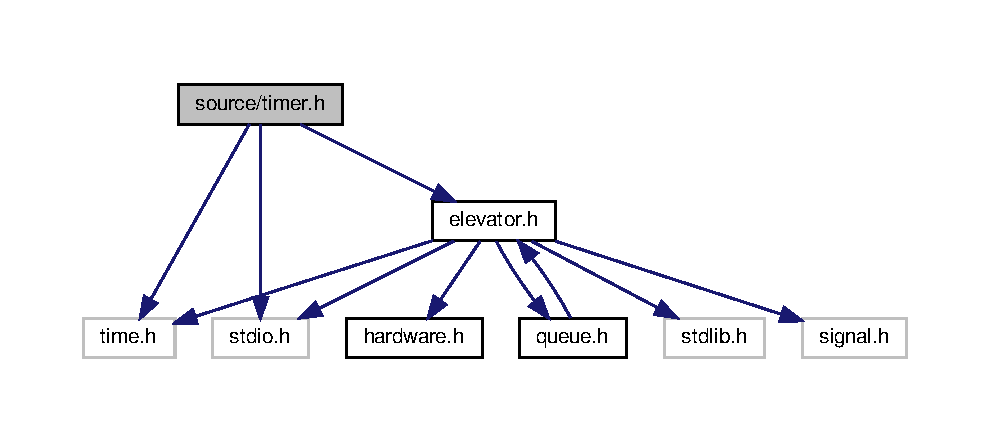
\includegraphics[width=350pt]{timer_8h__incl}
\end{center}
\end{figure}
This graph shows which files directly or indirectly include this file\+:
\nopagebreak
\begin{figure}[H]
\begin{center}
\leavevmode
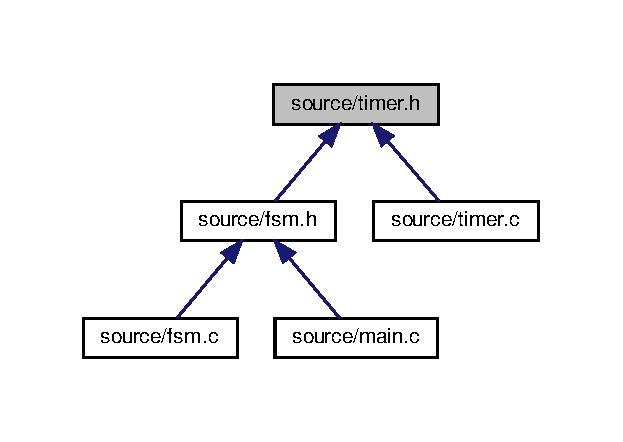
\includegraphics[width=319pt]{timer_8h__dep__incl}
\end{center}
\end{figure}
\subsection*{Macros}
\begin{DoxyCompactItemize}
\item 
\mbox{\Hypertarget{timer_8h_a5885ee63e43af9d199f9f29c09cb9c55}\label{timer_8h_a5885ee63e43af9d199f9f29c09cb9c55}} 
\#define {\bfseries D\+O\+O\+R\+\_\+\+T\+I\+ME}~3
\end{DoxyCompactItemize}
\subsection*{Functions}
\begin{DoxyCompactItemize}
\item 
void \hyperlink{timer_8h_aea3dcf2d3ef6743d9cb41914c5a5d72f}{start\+\_\+timer} (elevator $\ast$el)
\begin{DoxyCompactList}\small\item\em Starts the timer. \end{DoxyCompactList}\item 
int \hyperlink{timer_8h_af9fbb2e2157733d3cfb53784091a2d8e}{times\+\_\+up} (elevator $\ast$el)
\begin{DoxyCompactList}\small\item\em Checks if the time is up. \end{DoxyCompactList}\end{DoxyCompactItemize}


\subsection{Detailed Description}
Functions to keep the door open for a period of time. 



\subsection{Function Documentation}
\mbox{\Hypertarget{timer_8h_aea3dcf2d3ef6743d9cb41914c5a5d72f}\label{timer_8h_aea3dcf2d3ef6743d9cb41914c5a5d72f}} 
\index{timer.\+h@{timer.\+h}!start\+\_\+timer@{start\+\_\+timer}}
\index{start\+\_\+timer@{start\+\_\+timer}!timer.\+h@{timer.\+h}}
\subsubsection{\texorpdfstring{start\+\_\+timer()}{start\_timer()}}
{\footnotesize\ttfamily void start\+\_\+timer (\begin{DoxyParamCaption}\item[{elevator $\ast$}]{el }\end{DoxyParamCaption})}



Starts the timer. 


\begin{DoxyParams}[1]{Parameters}
\mbox{\tt in,out}  & {\em el} & The elevator. \\
\hline
\end{DoxyParams}


Definition at line 5 of file timer.\+c.

\mbox{\Hypertarget{timer_8h_af9fbb2e2157733d3cfb53784091a2d8e}\label{timer_8h_af9fbb2e2157733d3cfb53784091a2d8e}} 
\index{timer.\+h@{timer.\+h}!times\+\_\+up@{times\+\_\+up}}
\index{times\+\_\+up@{times\+\_\+up}!timer.\+h@{timer.\+h}}
\subsubsection{\texorpdfstring{times\+\_\+up()}{times\_up()}}
{\footnotesize\ttfamily int times\+\_\+up (\begin{DoxyParamCaption}\item[{elevator $\ast$}]{el }\end{DoxyParamCaption})}



Checks if the time is up. 


\begin{DoxyParams}[1]{Parameters}
\mbox{\tt in,out}  & {\em el} & The elevator. \\
\hline
\end{DoxyParams}
\begin{DoxyReturn}{Returns}
1 if the time is up, 0 if not. 
\end{DoxyReturn}


Definition at line 9 of file timer.\+c.


%--- End generated contents ---

% Index
\backmatter
\newpage
\phantomsection
\clearemptydoublepage
\addcontentsline{toc}{chapter}{Index}
\printindex

\end{document}
